\documentclass{beamer}

\setbeamertemplate{footline}[page number]
%\setbeamercovered{dynamic}
\usepackage{setspace}
\usepackage[T1]{fontenc}
\usepackage{graphicx}
\usepackage{amsmath}
\usepackage{amsfonts}
\usepackage{amssymb}
\usepackage{makeidx}
\usefonttheme{serif}
\usepackage{multirow}
\usepackage{booktabs} 
\usepackage{rotating}
\usepackage{color}
\usepackage{float}
%\usepackage[latin1]{inputenc}
%\usepackage[english]{babel}
%\usepackage{amsmath}
%\usepackage{amsfonts}
%\usepackage{amssymb}
%\usepackage{makeidx}
%\usepackage{graphicx}
\usepackage[latin1]{inputenc}
\usepackage[english]{babel}
\usepackage{amsmath}
\usepackage{amsfonts}

\usepackage{eurosym}
\usepackage{rotating}
\usepackage{multicol}
\setbeamertemplate{footline}[page number]
\date{}
\author{}
\institute{}

%%%%%%% Put these names back in the final version 
%\\Aswathy Rajendra Kurup\\Meenu Ajith}
%\institute{Department of Electrical and Computer Engineering\\The University of New Mexico}
\setbeamercovered{transparent}
\usepackage{setspace}
\usepackage{array}
\usepackage[T1]{fontenc}
\usepackage{graphicx}
\usepackage{amsmath}
\usepackage{amsfonts}
\usepackage{amssymb}
\usepackage{makeidx}
\usefonttheme{serif}
\usepackage{multirow}
\usepackage{booktabs} 
\usepackage{rotating}
\usepackage{color}
\usepackage{float}
\usepackage[latin1]{inputenc}
\usepackage[english]{babel}
\usepackage{amsmath}
\usepackage{amsfonts}
\usepackage{eurosym}
\usepackage{rotating}
\usepackage{multicol}
\usepackage{pythonhighlight}
\usepackage[normalem]{ulem}
\newcommand{\ba}{{\bf a}}
\newcommand{\bb}{{\bf b}}
\newcommand{\bc}{{\bf c}}
\newcommand{\bd}{{\bf d}}
\newcommand{\be}{{\bf e}}
\newcommand{\bbf}{{\bf f}}
\newcommand{\bg}{{\bf g}}
\newcommand{\bh}{{\bf h}}
\newcommand{\bi}{{\bf i}}
\newcommand{\bk}{{\bf k}}
\newcommand{\bl}{{\bf l}}
\newcommand{\bm}{{\bf m}}
\newcommand{\bn}{{\bf n}}
\newcommand{\bo}{{\bf o}}
\newcommand{\bp}{{\bf p}}
\newcommand{\bq}{{\bf q}}
\newcommand{\br}{{\bf r}}
\newcommand{\bs}{{\bf s}}
\newcommand{\bt}{{\bf t}}
\newcommand{\bu}{{\bf u}}
\newcommand{\bv}{{\bf v}}
\newcommand{\bw}{{\bf w}}
\newcommand{\bx}{{\bf x}}
\newcommand{\by}{{\bf y}}
\newcommand{\bz}{{\bf z}}

\newcommand{\bA}{{\bf A}}
\newcommand{\bB}{{\bf B}}
\newcommand{\bC}{{\bf C}}
\newcommand{\bE}{{\bf E}}
\newcommand{\bG}{{\bf G}}
\newcommand{\bH}{{\bf H}}
\newcommand{\bI}{{\bf I}}
\newcommand{\bK}{{\bf K}}
\newcommand{\bL}{{\bf L}}
\newcommand{\bM}{{\bf M}}
\newcommand{\bO}{{\bf O}}
\newcommand{\bQ}{{\bf Q}}
\newcommand{\bR}{{\bf R}}
\newcommand{\bS}{{\bf S}}
\newcommand{\bT}{{\bf T}}
\newcommand{\bV}{{\bf V}}
\newcommand{\bW}{{\bf W}}
\newcommand{\bX}{{\bf X}}
\newcommand{\bY}{{\bf Y}}
\newcommand{\bZ}{{\bf Z}}
\newcommand\uptocnt{\stackrel{\mathclap{\normalfont\mbox{c}}}{\propto}}
\newcommand{\bpt}{{\bf pt}}
\newcommand{\bpl}{{\bf pl}}
\newcommand{\bdp}{{\bf dp}}
\newcommand{\btemp}{{\bf temp}}

\newcommand{\bmu}{{\boldsymbol \mu}}
\newcommand{\bSigma}{{\boldsymbol \Sigma}}
\newcommand{\bsigma}{{\boldsymbol \sigma}}
\newcommand{\bvarPhi}{{\boldsymbol \varPhi}}
\newcommand{\bvarphi}{{\boldsymbol \varphi}}
\newcommand{\bPhi}{{\boldsymbol \Phi}}
\newcommand{\bdelta}{{\boldsymbol \delta}}
\newcommand{\bZero}{{\bf 0}}
\newcommand{\bOne}{{\bf 1}}
\newcommand{\balpha}{{\boldsymbol \alpha}}
\newcommand{\bAlpha}{{\boldsymbol A}}
\newcommand{\btheta}{{\boldsymbol \theta}}

\newcommand{\softmax}{\text{softmax}}
\newcommand{\diag}{\text{diag}}
\newcommand{\sinc}{\mathrm{sinc}}
\newcommand{\argmin}{\mathop{\mathrm{argmin}}}
\newcommand{\infl}{\eta}
\newcommand{\Ind}{\mathrm{I}}
\newcommand{\Real}{\mathbb R}
\newcommand{\Intg}{\mathbb Z}
\newcommand{\Complex}{\mathbb C}
\newcommand{\Natural}{\mathbb N}
\newcommand{\Fourier}[1]{\mathcal{F} \{#1\}}
%\newcommand{\ii}{\mathbbm{i}}
\newcommand{\bphi}{\boldsymbol{\mathit{\phi}}}

\newcommand{\hs}{\hspace{2pt}}
\newcommand{\sign}{\text{sign}}
\author{Manel Mart\'inez-Ram\'on\\Meenu Ajith\\Aswathy Rajendra Kurup}

\usetheme{Madrid}
\usecolortheme{beaver}
\usepackage{tikz}
\usetikzlibrary{fit,arrows,calc,positioning}
\usepackage{listings}
\usepackage{xcolor}
\usepackage{emerald} 
\usepackage[T1]{fontenc} 
\usepackage{verbatim}
\usepackage{graphicx}
\usepackage{epsfig}
\usepackage{psfrag}
\usepackage[english]{babel}
\usepackage{listings}
\usepackage{courier}
\usepackage{color}
 \usepackage{vwcol} 
 \usepackage[english]{babel} % To obtain English text with the blindtext package
\usepackage{blindtext}
\definecolor{codegreen}{rgb}{0,0.6,0}
\definecolor{codegray}{rgb}{0.5,0.5,0.5}
\definecolor{codepurple}{rgb}{0.58,0,0.82}
\definecolor{backcolour}{rgb}{0.95,0.95,0.92}

\lstdefinestyle{mystyle}{
  backgroundcolor=\color{backcolour},   commentstyle=\color{codegreen},
  keywordstyle=\color{magenta},
  numberstyle=\tiny\color{codegray},
  stringstyle=\color{codepurple},
  basicstyle=\ttfamily\footnotesize,
  breakatwhitespace=false,         
  breaklines=true,                 
  captionpos=b,                    
  keepspaces=true,                 
  numbers=left,                    
  numbersep=5pt,                  
  showspaces=false,                
  showstringspaces=false,
  showtabs=false,                  
  tabsize=2
}
\lstset{style=mystyle}

%% Stuff for movies

% %\newcommand{\bt}{{\bf t}}
% \newcommand{\br}{{\bf r}}
% \newcommand{\bs}{{\bf s}}
% \newcommand{\by}{{\bf y}}
% \newcommand{\bz}{{\bf z}}
% \newcommand{\bx}{{\bf x}}
% \newcommand{\bw}{{\bf w}}
% \newcommand{\be}{{\bf e}}
% \newcommand{\bbf}{{\bf f}}
% \newcommand{\bb}{{\bf b}}
% \newcommand{\bd}{{\bf d}}
% \newcommand{\bA}{{\bf A}}
% \newcommand{\bB}{{\bf B}}
% \newcommand{\bL}{{\bf L}}
% \newcommand{\bM}{{\bf M}}

% \newcommand{\bC}{{\bf C}}
% \newcommand{\bI}{{\bf I}}
% \newcommand{\bK}{{\bf K}}
% \newcommand{\bk}{{\bf k}}
% \newcommand{\bT}{{\bf T}}
% \newcommand{\bV}{{\bf V}}
% \newcommand{\bW}{{\bf W}}
% \newcommand{\bX}{{\bf X}}
% \newcommand{\bY}{{\bf Y}}
% \newcommand{\bZ}{{\bf Z}}
% \newcommand{\bm}{{\bf m}}
% \newcommand{\bpt}{{\bf pt}}
% \newcommand{\bpl}{{\bf pl}}
% \newcommand{\bdp}{{\bf dp}}
% \newcommand{\btemp}{{\bf temp}}
% \newcommand{\bl}{{\bf l}}
% \newcommand{\bu}{{\bf u}}
% \newcommand{\bmu}{{\boldsymbol \mu}}
% \newcommand{\bSigma}{{\boldsymbol \Sigma}}
% \newcommand{\bLambda}{{\boldsymbol \Lambda}}

% \newcommand{\bsigma}{{\boldsymbol \sigma}}
% \newcommand{\bvarphi}{{\boldsymbol \varPhi}}
% \newcommand{\btheta}{{\boldsymbol \theta}}
% \newcommand{\bZero}{{\bf 0}}
% \newcommand{\balpha}{{\boldsymbol \alpha}}
% \newcommand{\bpi}{{\boldsymbol \pi}}
% \newcommand{\bxi}{{\boldsymbol \xi}}
% \newcommand{\bdelta}{{\boldsymbol \delta}}
\lstset{
	language=Python,
	basicstyle=\footnotesize\ttfamily\color{black},
	commentstyle = \footnotesize\ttfamily\color{red},
	keywordstyle=\footnotesize\ttfamily\color{blue},
	stringstyle=\footnotesize\ttfamily\color{black},
%	columns=fixed,
%	numbers=left,    
	numberstyle=\tiny,
	stepnumber=1,
	numbersep=5pt,
	tabsize=1,
	extendedchars=true,
	breaklines=true,            
	frame=b,         
	showspaces=false,
	showtabs=true,
	xleftmargin=6pt,
	framexleftmargin=6pt,
	framexrightmargin=2pt,
	framexbottommargin=4pt,
	showstringspaces=false      
}

\lstloadlanguages{
         Python
}

%\graphicspath{ {./images/} }  % Figures path - used in graphicx

%\selectcolormodel{cmyk}

\mode<presentation>

\newcommand{\dred}{darkred!90!black}
\newcommand{\written}{\ECFJD\textcolor{cyan!50!white}}
\newcommand{\hlight}{\textcolor{\dred}}
\newcommand{\Ex}{\textcolor{\dred}{Ex. }}

% remove navigation symbols in full screen mode
\setbeamertemplate{navigation symbols}{}  
\setbeamertemplate{blocks}[rounded][shadow=false]
\setbeamercolor{note page}{fg=black}

\setbeamercolor{title}{fg=\dred}
\setbeamercolor{frametitle}{fg=white}
\setbeamercolor{frametitle}{bg=\dred}
\setbeamercolor{structure}{fg=black,bg=white}
\setbeamercolor{background canvas}{bg=white,fg=black}
\setbeamercolor{normal text}{fg=black,bg=white}
\setbeamercolor{item}{fg=red!80!black,bg=white!}
\addtobeamertemplate{block begin}{\setbeamercolor{block title}{fg=white,bg=\dred}
\setbeamercolor{block body}{fg=white,bg=gray}}{}


%\author{Manel Mart\'inez Ram\'on}
\title{\textbf{AI in an nutshell}}
\subtitle{}

\date{}

\addtobeamertemplate{frametitle}{}{}

\section{Manel Mart\'inez-Ram\'on}
\subsection{\textbf{What is} (wrong with) \textbf{AI?}}
\begin{document}
\maketitle

\begin{frame}{Nobel Prize in Physics 2024}
\centering
        \includegraphics[scale=0.27]{pics/HINTON_HOPFIELD.png}
\end{frame}

\begin{frame}{Nobel Prize in Physics 2024}
\begin{multicols}{2}
\begin{itemize}
    \item IA is everywhere. 
    \item What is its relation with physics?
    \begin{enumerate}
    \item  Developed from models known in physics
    \item  Used to solve problems in physics
    \item  IA revolutionized the World
\end{enumerate}
\end{itemize}


\columnbreak

\centering
\includegraphics[width=0.35\textwidth]{pics/neurons.jpeg}
    



\end{multicols}

\end{frame}

\begin{frame}{From computers to reasoning}
    \includegraphics[scale = 0.15]{pics/computer.png}  

\vspace{-0.1in}
\hspace{2in}
    \includegraphics[scale=0.15]{pics/kasparov.png}
\end{frame}


\begin{frame}{Computers and complex tasks}
\centering
\includegraphics[scale=0.28]{pics/robot_cooking.jpg}
\end{frame}

\begin{frame}{Hand me a glass}
\centering
\includegraphics[scale=0.7]{pics/glasses.jpg}
\end{frame}

\begin{frame}{The learning concept}
\centering
\includegraphics[scale=0.4]{pics/turing.jpg}

Alan Turing (1912-1954)
\end{frame}


\begin{frame}{What is Artificial Intelligence?}
\begin{center}
In 1956, John McCarthy organized a conference in Dartmouth College ``to proceed on the basis of the conjecture that every aspect of learning or any other feature of intelligence can in principle be so precisely described that a machine can be made to simulate it."
\end{center}

\begin{footnotesize}{McCarthy,  Minsky, Rochester and Shannon, ``\emph{A proposal for the Darmouth Summer Research Project on Artificial Intelligence}'', 1956.}
\end{footnotesize}

\vspace{0.5cm}
\centering
Sixty seven years and six months later,\\ we still do not exactly know what it is. 

\end{frame}

\begin{frame}{The neuron}
\begin{multicols}{3}

\includegraphics[scale=0.935]{pics/golgi.jpg}
Camilo Golgi (1843-1926)
\columnbreak

\includegraphics[scale=2]{pics/cajal.jpg}
Santiago Ram\'on  y Cajal (1852-1934)

\columnbreak

\includegraphics[scale=0.18]{pics/Fig_retine.png}

Santiago Ram\'on y Cajal, Histologie Du Syst\`eme Nerveux de l'Homme et Des Vert\`ebr\`es, Maloine, Paris, 1911, 
\end{multicols}

C. Golgi (Italy) and S. Ram\'on y Cajal (Spain) were awarded the 1906 Nobel Prize in Physiology and Medicine. 
\end{frame}


\begin{frame}{Inception of the artificial neuron}
\begin{itemize}
    \item McCulloch and Pitts, 1943
\begin{center}
\includegraphics[scale=0.15]{pics/McCullochPittsPaper.png}~~~~~~~~
\includegraphics[scale=0.15]{pics/McCullochPitts.png}
\end{center}

\item Hebb, 1949

\begin{center}
\includegraphics[scale=0.25]{pics/hebb_synapsis.png}
\includegraphics[scale=0.15]{pics/Donald Hebb.jpg}
\end{center}
\end{itemize}
\end{frame}

\begin{frame}{The perceptron}
\begin{itemize}
\item Rosemblatt, 1958
\end{itemize}
\begin{center}
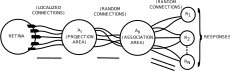
\includegraphics[scale=0.3]{pics/rosemblattsPERCEPTRON.pdf}
\includegraphics[scale=0.15]{pics/Rosenblatt.jpg}
\end{center}

\begin{center}
\includegraphics[scale=0.25]{pics/NYT_header.png}\\
\includegraphics[scale=0.33]{pics/Mark_I_perceptron.jpg}
\includegraphics[scale=0.23]{pics/NYT1958-07-13.png}
\end{center}
\end{frame}


\begin{frame}{Hopfield, 1982}
\centering\includegraphics[scale=0.4]{pics/Hopfield_paper.png}

Hopfield uses the collective behavior of matter to generate computational capacity.
\end{frame}

\begin{frame}{Hinton, 1983}
    \centering
    \includegraphics[scale=0.4]{pics/HintonPaper.png}

Hinton uses concepts of thermodynamics to train Hopfield's networks: the Boltzmann distribution. It leads to the concept of collective behavior.
\end{frame}
\begin{frame}{The neural network}

\begin{center}
    \includegraphics[scale=0.3]{pics/mlp.pdf}\\
       \includegraphics[scale=0.18]{pics/NN_relu1.pdf}
       \includegraphics[scale=0.18]{pics/spiral.pdf}
\end{center}

Werbos (1974, 1988);  Rumelhart, Hinton \& Williams (1986). 
\end{frame}

\begin{frame}{Initial difficulties of AI}
\begin{center}
\includegraphics[scale=0.4]{pics/old_computing.pdf}
\end{center}
\end{frame}


\begin{frame}{Convolutional neural networks}
 David Hubel and Torsten Wiesel (1981 Nobel Prize in Medicine), 1958.
\begin{center}
   \includegraphics[scale=0.3]{pics/Hubel_Wiesel.pdf}
\end{center}

Yan LeCun (2018 Turing Award), 1989

\begin{center}
    \includegraphics[scale=0.25]{pics/LeCunLicenced.png}\includegraphics[scale=0.35]{pics/Lecun.jpeg}
\end{center}

    
\end{frame}






\begin{frame}{Recurrent Neural Networks}
Elman, 1972, Hochreiter, 1997, Sutskever, 2012

\begin{center}
\includegraphics[scale=0.1]{pics/rnn_unrolled.pdf}
\includegraphics[scale=0.2]{pics/google_translate.png}
\end{center}
\vspace{-0.5 cm}


\end{frame}


\begin{frame}{AI tools}

\begin{center}
    \includegraphics[scale=0.4]{pics/AI_tools.pdf}
\end{center}    
\end{frame}

\begin{frame}{Self attention and transformers}
    \begin{center}
        \includegraphics[scale=0.5]{pics/self_attention.pdf}
    \end{center}
\end{frame}
\end{document}